\begin{frame}
\frametitle{Aufgabe 4}
\framesubtitle{}
    \begin{itemize}
        \item Durch kompliziertere Schaltungen können schärfere
        Frequenztrennungen erreicht werden
    \end{itemize}
\end{frame}
\begin{frame}
\frametitle{Aufgabe 4}
\framesubtitle{Tiefpass 2. Ordnung}
\begin{figure}[H]
\begin{center}
        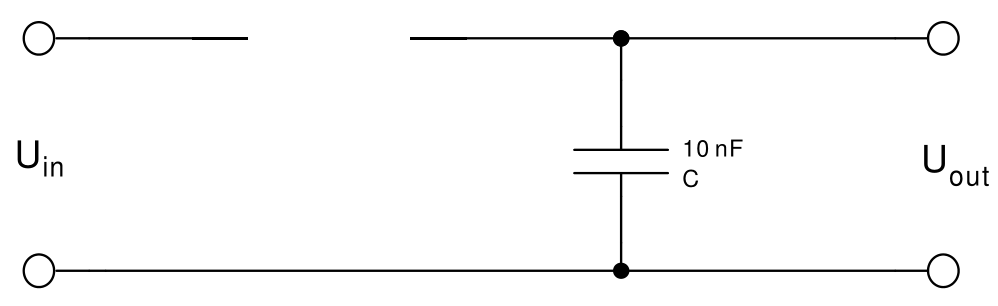
\includegraphics[scale=0.2]{./img/4a_tiefpass_1.png}
\end{center}
\end{figure}
\end{frame}
\begin{frame}
\frametitle{Aufgabe 4}
\framesubtitle{Tiefpass 2.Ordnung}
\begin{figure}[H]
\begin{center}
        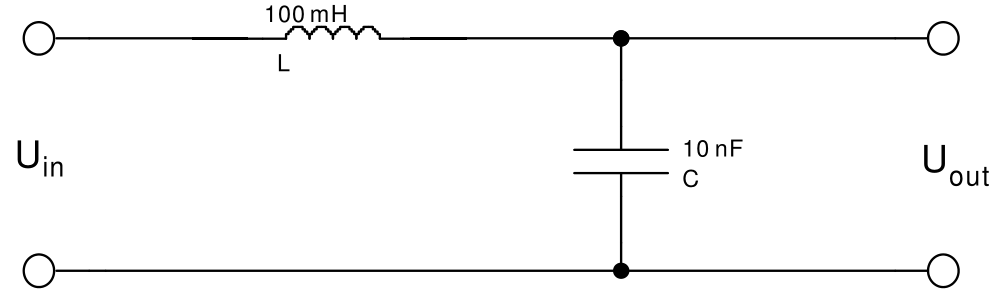
\includegraphics[scale=0.2]{./img/4a_tiefpass_2.png}
\end{center}
\end{figure}
\begin{itemize}
    \item Einbau von Spule
\end{itemize}
\begin{equation*}
    \frac{U_{out}}{U_{in}} = \frac{1}{1-\omega^2 L C}
\end{equation*}
\end{frame}
